\documentclass{article}
\usepackage{graphicx}
\usepackage{float}
\title{Circgraph: a Galaxy tool for Circos-enabled genomic data visualization}
\author{Stephen Crosby}
\begin{document}
\maketitle
\section*{Abstract}
Advancements in molecular biology in the past two decades have led to the acquisition of
unprecedented amounts of DNA sequence data, but the visualization of this data and its
interpretation remain important challenges to the scientific community. Several approaches to
create informative plots of sequence data have been devised in response to these challenges, 
including Circos: graphics software which allows users to design circular plots highlighting
interesting genomic features and comparing different organismal genomes. In order to facilitate sequence analyses and Circos plot development, an online Galaxy tool was developed which
will enable scientists to incorporate bioinformatics techniques into their work while bypassing the learning curve associated with command-line tool usage. The tool, which has both command-line and web-based interfaces, allows users broad cosmetic control over the appearance of produced Circos plots, includes methods for parsing and interpreting several common file types used for visualizing genomic data, and supports most the principal track types present in the Circos suite. This new interface to the existing Circos software will enable life scientists to easily and efficiently create informative views of a variety of sequence data formats.

\section*{Introduction}
Macromolecular sequencing has been the underpinning of many crucial developments in modern biomedical research, and since the advent of sequencing technology in the 1970s, improvements in experimental techniques have enabled scientists to produce ever-increasing amounts of nucleic and amino acid sequence data. The increasing popularity of these high-throughput molecular techniques has challenged the bioinformatics community to develop new solutions for data-management, statistical analysis, and genome annotation. Visualizing this newly produced genomic data remains an important obstacle to both the effective utilization of sequence data as well as the continued growth and adoption of bioinformatic methods by new scientists.  

Several responses have been made to the challenge of visualization, but one of the most successful has been Circos: a software suite produces circular analogs of classical graphics and promises to facilitate the comparison of genomes with two-dimensional data tracks and links.

Another obstacle to the growth of bioinformatics within classical scientific disciplines is the learning curve associated with the use of these new, computerized tools; 21st century software development initiatives such as the Galaxy project are lowering the barriers between established wet-lab scientists and cutting edge computational techniques by eschewing the traditional command-line interface in favor of broadly-accessible, user-friendly web apps.


\section*{Methods}
Developed in 2004, the Circos visualization software suite manages the creation of circular plots of genomic datasets using text-based configuration files; with a specific format analogous to the XML standard, configuration files have the potential to be extensibly generated by exploiting existing software.    

An XML-driven Galaxy tool through which users can specify data to be used in tracks and cosmetic parameters for the Circos plots was developed with Jinja2, and the core of the new Galaxy tool is a Python script which manages these parameters and writes them to configuration files consistent with the Circos specification. 

\section*{Results and Discussion}

In order to facilitate the visualization of high-throughput genomic data in several file formats, Circgraph, a web-based Galaxy tool exploiting the existing Circos software suite freely available online, was developed. Currently, the program has been implemented as a command-line tool in order to allow the user to pass data files dictating the composition of data tracks, but the software support required for users to set parameter values from the online Galaxy interface have already been deveoped.

Circgraph can accept and parse several common genomic file types including fasta, bigWig, gff3, and ProgressiveMauve backbone files into text files suitable for interpretation by Circos.

Circgraph handles several of the principal data track types available through Circos including 2D data tracks such as heatmaps, histograms, and scatterplots, highlights indicating specific regions of interest within sequence data, and links associating homologous runs within two sequences.

\begin{figure}[H]
\centering
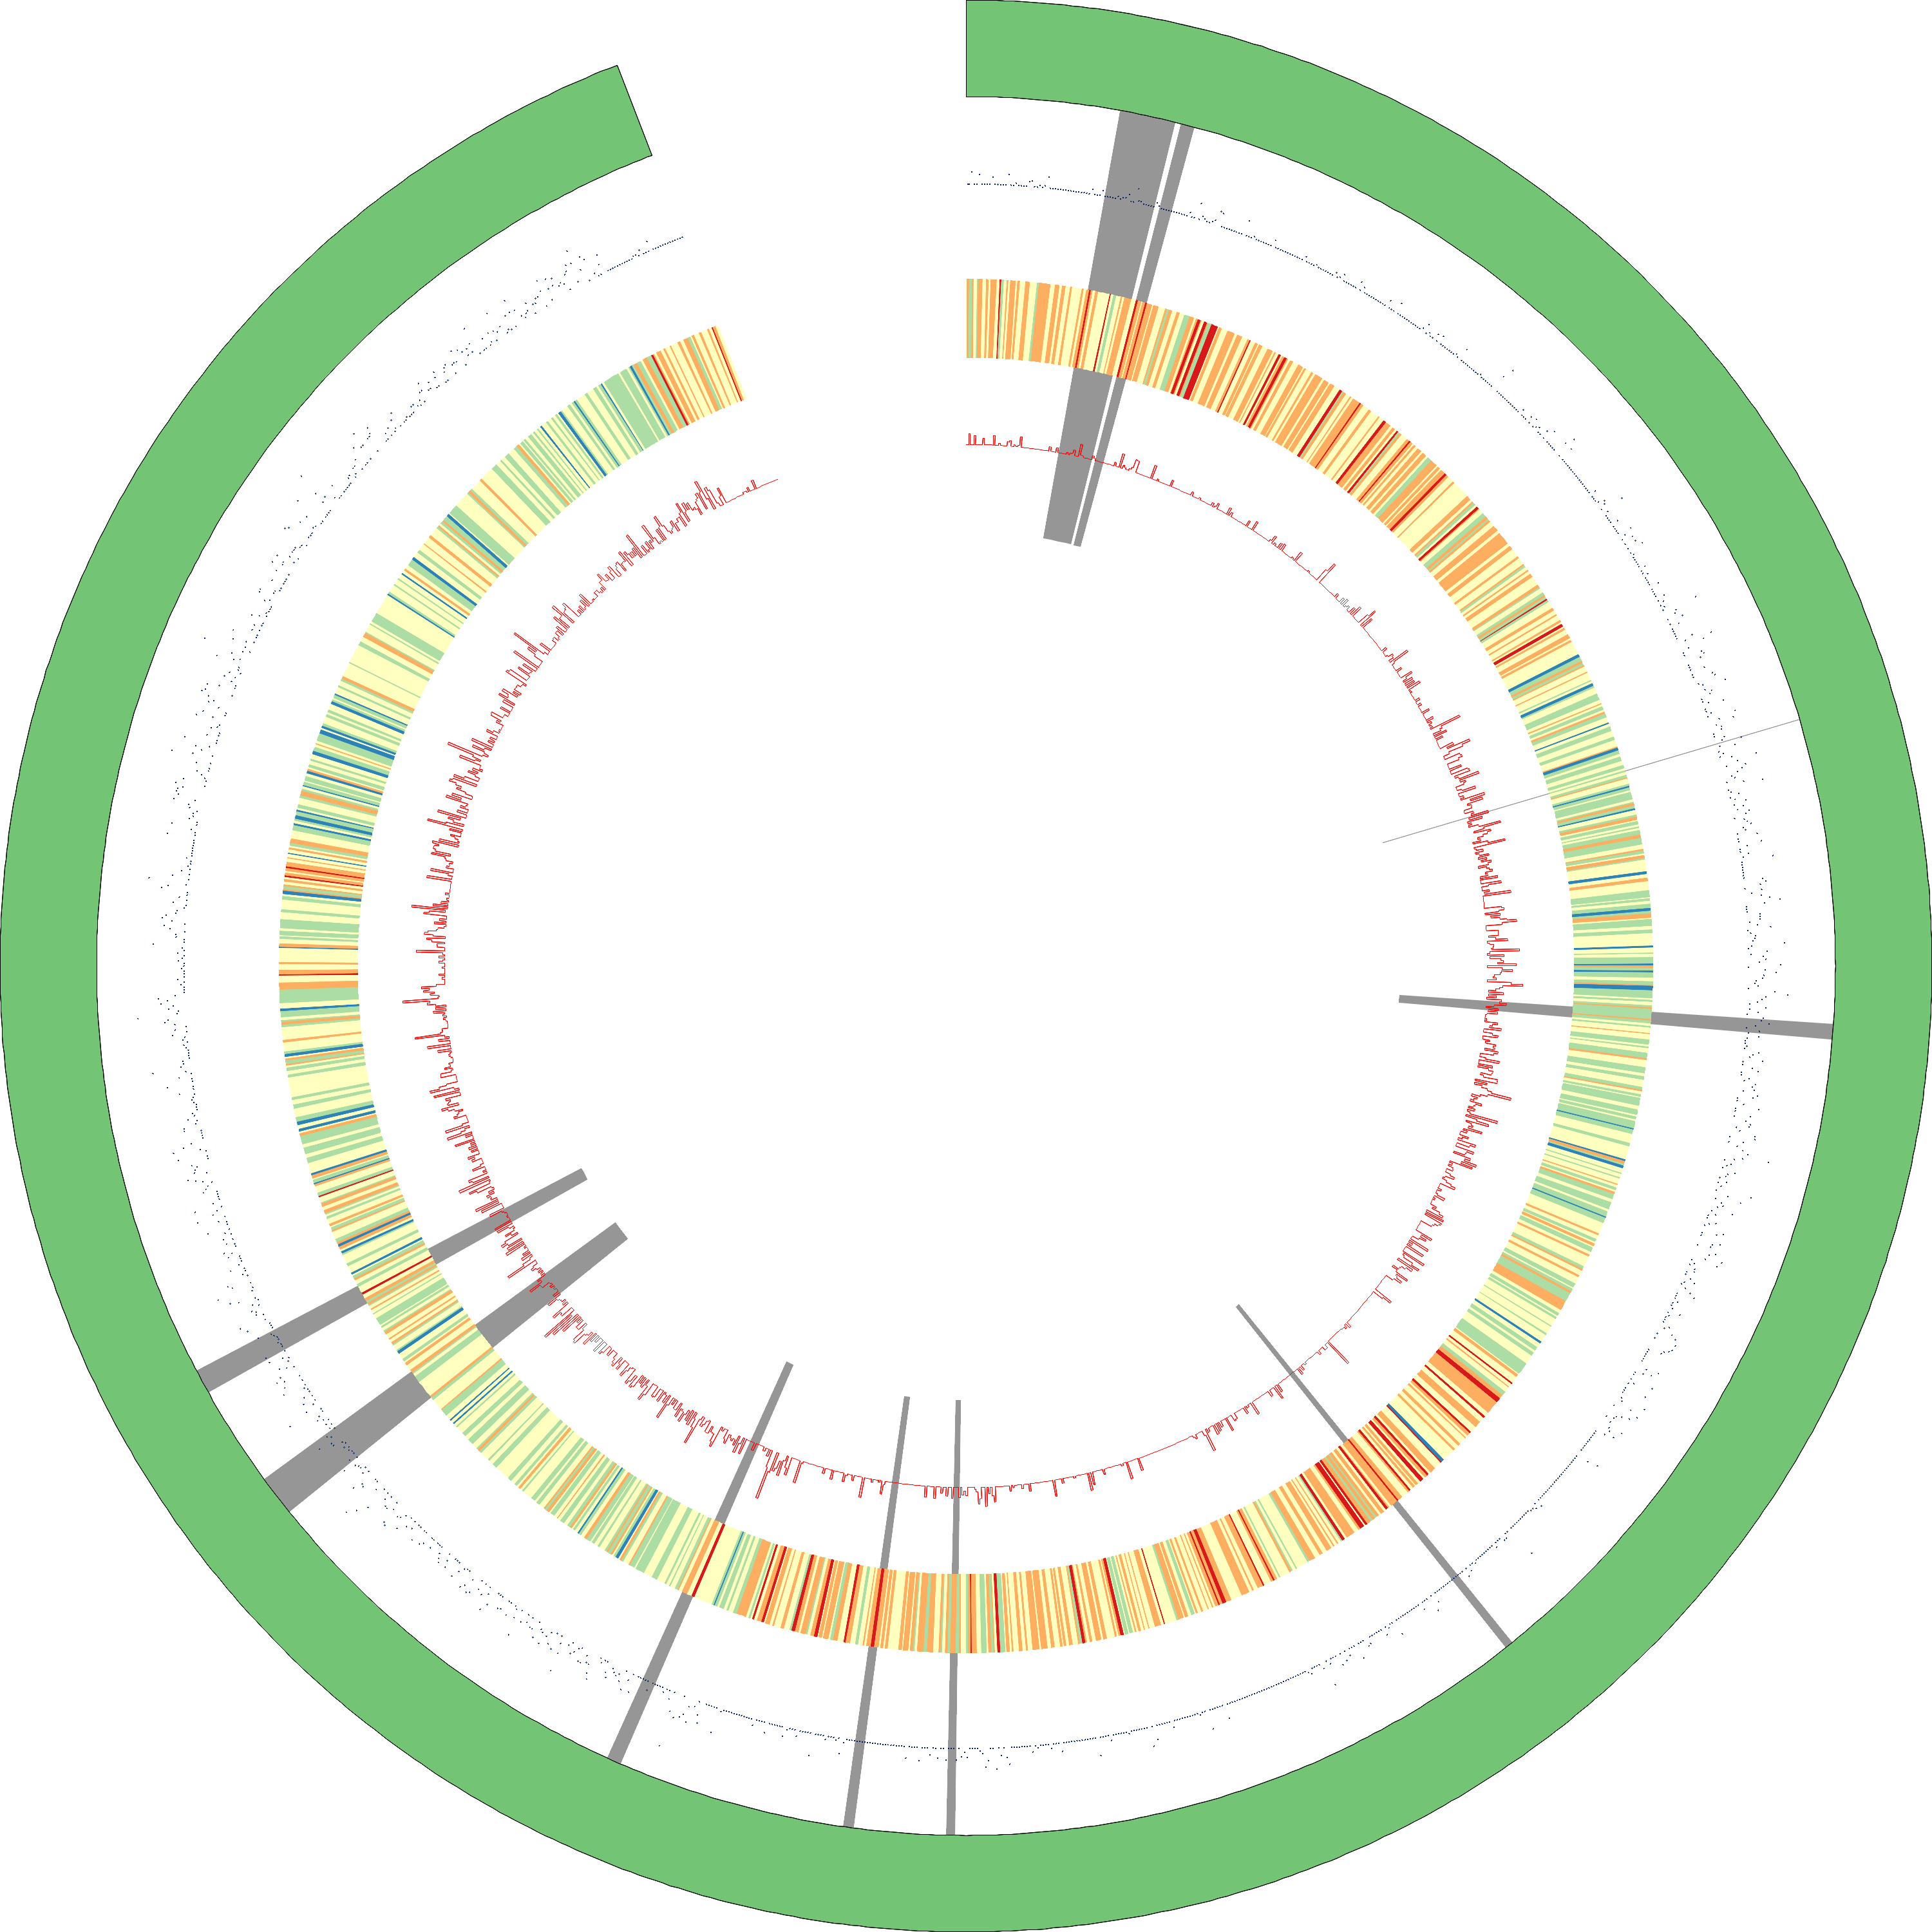
\includegraphics[scale=0.1]{./results/hilite.png}
\caption{Circgraph allows users to create several native Circos data track types, including histograms, heatmaps, and scatterplots. Highlights can also be added to accentuate certain regions; here, highlights are shown in grey.}
\end{figure}

\begin{figure}[H]
\centering
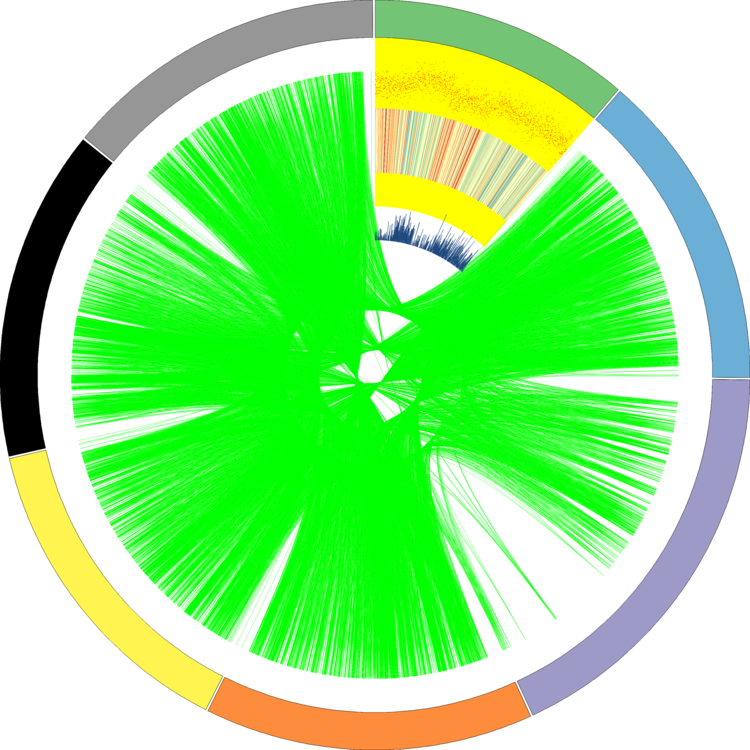
\includegraphics[scale=0.1]{./links.png}
\caption{Circgraph supports arrangement of multiple chromosomes within a plot and can create links between chromosomes if provided with ProgressiveMauve-generated backbone files.}
\end{figure}

Several challenges remain to the effective use of Circos for genomic data visualization; in particular, continuing improvements to existing algorithms and workflows which can separate statistically-significant, biologically-relevant data from the ambient dataset will improve the signal-to-noise ratio of Circos plots.

\begin{figure}[H]
\centering
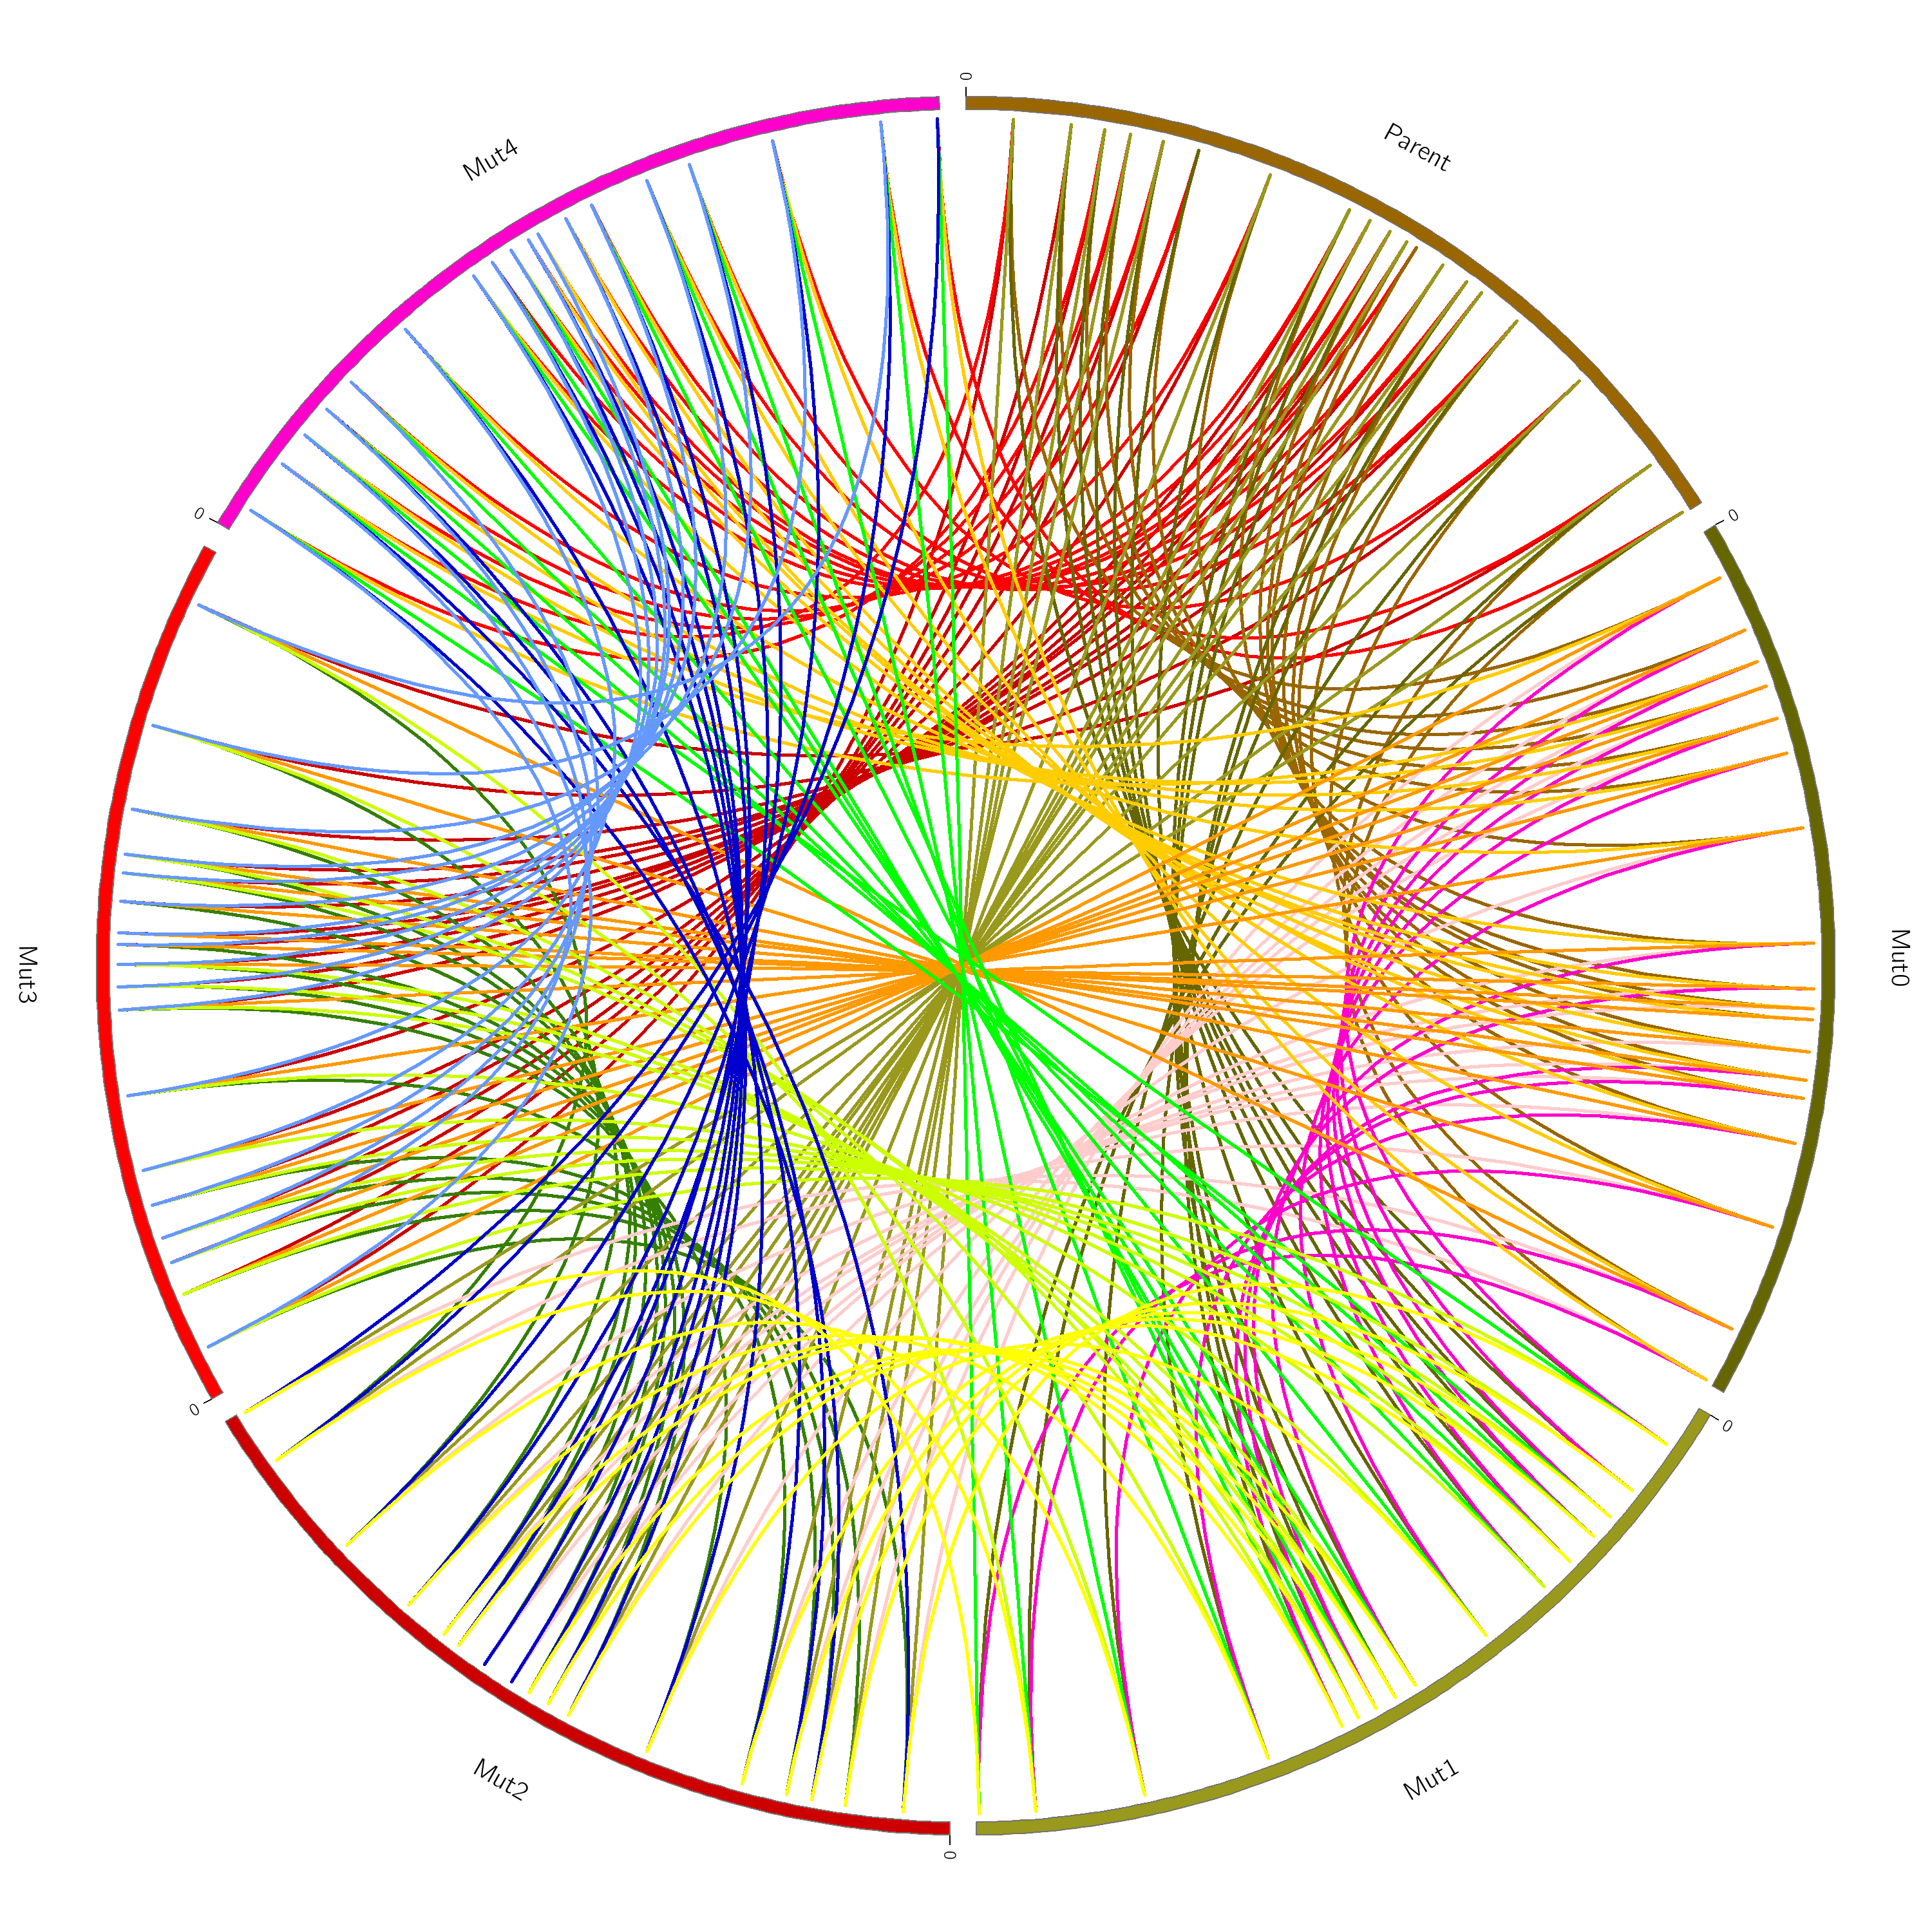
\includegraphics[scale=0.1]{./Generated_Data_Non_Ribbon.png}
\caption{Even when color-coded, unstratified link data is not suitable for creating easily interpreted graphics. Currently, Circgraph does not support rules for data stratification as the graphic is being created.}
\end{figure}

\begin{figure}[H]
\centering
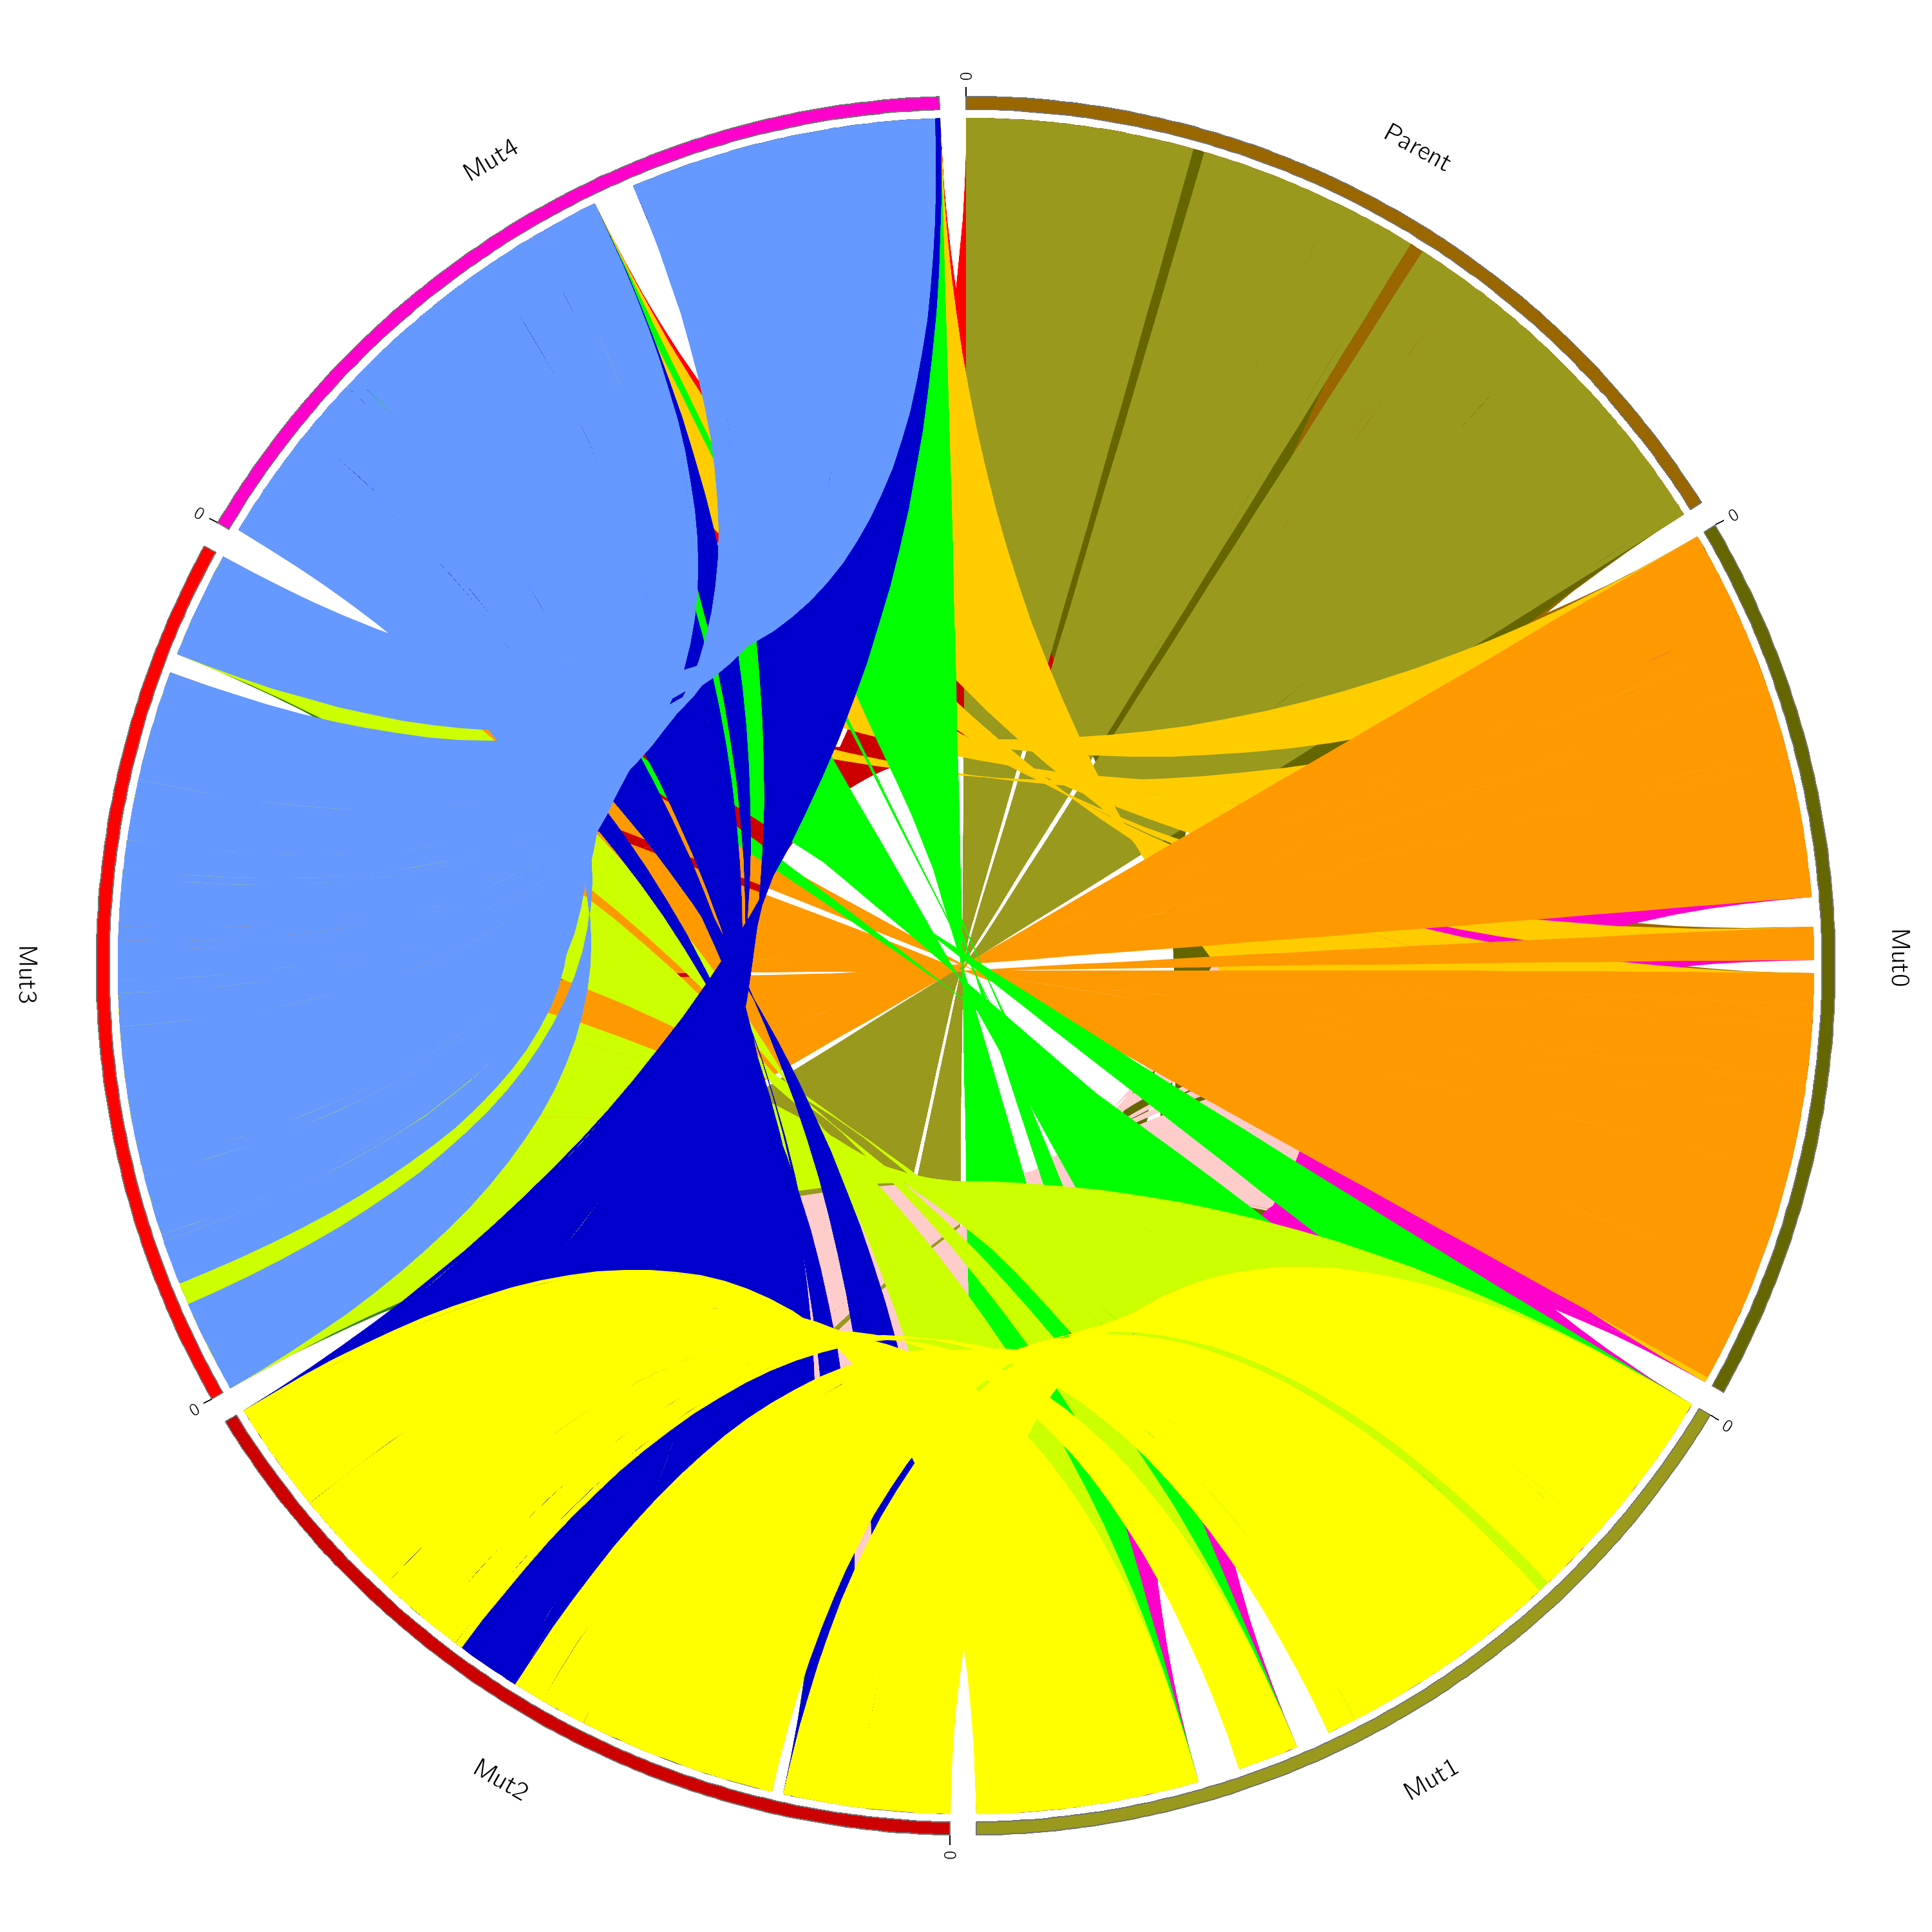
\includegraphics[scale=0.1]{./Generated_Color_Fixes.png}
\caption{Coarser link data poses its own interpretive difficulties; larger, opaque ribbon links can obscure each other.}
\end{figure}

Continued development of Circgraph will be required in order to capture the full span of features offered by the Circos visualization software, and guided, intelligent creation of high-quality graphics may be possible with additional code improvements. 

\section*{References}
\begin{enumerate}
\item
\end{enumerate}

\end{document}
